
%% bare_conf.tex
%% V1.3
%% 2007/01/11
%% by Michael Shell
%% See:
%% http://www.michaelshell.org/
%% for current contact information.
%%
%% This is a skeleton file demonstrating the use of IEEEtran.cls
%% (requires IEEEtran.cls version 1.7 or later) with an IEEE conference paper.
%%
%% Support sites:
%% http://www.michaelshell.org/tex/ieeetran/
%% http://www.ctan.org/tex-archive/macros/latex/contrib/IEEEtran/
%% and
%% http://www.ieee.org/

%%*************************************************************************
%% Legal Notice:
%% This code is offered as-is without any warranty either expressed or
%% implied; without even the implied warranty of MERCHANTABILITY or
%% FITNESS FOR A PARTICULAR PURPOSE! 
%% User assumes all risk.
%% In no event shall IEEE or any contributor to this code be liable for
%% any damages or losses, including, but not limited to, incidental,
%% consequential, or any other damages, resulting from the use or misuse
%% of any information contained here.
%%
%% All comments are the opinions of their respective authors and are not
%% necessarily endorsed by the IEEE.
%%
%% This work is distributed under the LaTeX Project Public License (LPPL)
%% ( http://www.latex-project.org/ ) version 1.3, and may be freely used,
%% distributed and modified. A copy of the LPPL, version 1.3, is included
%% in the base LaTeX documentation of all distributions of LaTeX released
%% 2003/12/01 or later.
%% Retain all contribution notices and credits.
%% ** Modified files should be clearly indicated as such, including  **
%% ** renaming them and changing author support contact information. **
%%
%% File list of work: IEEEtran.cls, IEEEtran_HOWTO.pdf, bare_adv.tex,
%%                    bare_conf.tex, bare_jrnl.tex, bare_jrnl_compsoc.tex
%%*************************************************************************

% *** Authors should verify (and, if needed, correct) their LaTeX system  ***
% *** with the testflow diagnostic prior to trusting their LaTeX platform ***
% *** with production work. IEEE's font choices can trigger bugs that do  ***
% *** not appear when using other class files.                            ***
% The testflow support page is at:
% http://www.michaelshell.org/tex/testflow/



% Note that the a4paper option is mainly intended so that authors in
% countries using A4 can easily print to A4 and see how their papers will
% look in print - the typesetting of the document will not typically be
% affected with changes in paper size (but the bottom and side margins will).
% Use the testflow package mentioned above to verify correct handling of
% both paper sizes by the user's LaTeX system.
%
% Also note that the "draftcls" or "draftclsnofoot", not "draft", option
% should be used if it is desired that the figures are to be displayed in
% draft mode.
%
\documentclass[conference]{IEEEtran}
% Add the compsoc option for Computer Society conferences.
%
% If IEEEtran.cls has not been installed into the LaTeX system files,
% manually specify the path to it like:
% \documentclass[conference]{../sty/IEEEtran}





% Some very useful LaTeX packages include:
% (uncomment the ones you want to load)



\ifCLASSINFOpdf
  \usepackage[pdftex]{graphicx}
  % declare the path(s) where your graphic files are
  % \graphicspath{{../pdf/}{../jpeg/}}
  % and their extensions so you won't have to specify these with
  % every instance of \includegraphics
  % \DeclareGraphicsExtensions{.pdf,.jpeg,.png}




%\hyphenation{op-tical net-works semi-conduc-tor}
\usepackage{authblk}

\begin{document}
%
% paper title
% can use linebreaks \\ within to get better formatting as desired
\title{Decision Tree Classifiers with GA based feature
selectors}


% author names and affiliations
% use a multiple column layout for up to three different
% affiliations

\author[1]{Mrs. Shantha Rangaswamy\thanks{shantharangaswamy@rvce.edu.in}}
\author[2]{Dr. Shobha G\thanks{shobhag@rvce.edu.in}}
\author[3]{Dr.B.L.Shivakumar\thanks{shivakumarbl@rvce.edu.in}}
\author[4]{Samir Sheriff\thanks{samiriff@gmail.com}}
\author[5]{Satvik N\thanks{nsatvik@gmail.com}}

\affil[1]{shantharangaswamy@rvce.edu.in, Assistant Professor, Department of Computer Science, RV College of Engineering.}
\affil[2]{shobhag@rvce.edu.in, Dean PG Studies (CSE and ISE), Department of Computer Science, RV College of Engineering.}
\affil[3]{shivakumarbl@rvce.edu.in, HOD, Department of Civil Engineering, RV College of Engineering.}
\affil[4]{samiriff@gmail.com, 7th semester BE, Department of Computer Science, RV College of Engineering.}
\affil[5]{nsatvik@gmail.com, 7th semester BE, Department of Computer Science, RV College of Engineering.}


%\author{
%\IEEEauthorblockN{Dr. N. K. Cauvery}
%\IEEEauthorblockA{Professor\\ Department of Computer Science\\RV College of Engineering\\
%Email: cauverynk@rvce.edu.in}
%\and
%\IEEEauthorblockN{Sandhya S}
%\IEEEauthorblockA{Assistant Professor\\ Department of Computer Science\\RV College of Engineering\\
%Email:sandhya.sampangi@rvce.edu.in}
%\and 
%\IEEEauthorblockN{Satvik N}
%\IEEEauthorblockA{BE 7 semester\\ Department of Computer Science\\RV College of Engineering\\
%Email:nsatvik@gmail.com}
%\and
%\IEEEauthorblockN{Vaishakh BN}
%\IEEEauthorblockA{BE 7 semester\\ Department of Computer Science\\RV College of Engineering\\
%Email: vaishakhbn@gmail.com}
%
%}
%\author{
%    Dr. N. K. Cauvery\\
%	Professor\\
%	Department of Computer Science\\
%	RV College of Engineering
%  \and
%    Ms. Sandhya S.
%    Assistant Professor\\
%	Department of Computer Science\\
%	RV College of Engineering
%    \and
%    Satvik N\\
%    Student 7 semester\\
%	Department of Computer Science\\
%    email@edu
%    \and
%    Fourth Author\\
%    Department of Computer Science\\
%	RV College of Engineering
%    email@edu
%}



% make the title area
\maketitle


\begin{abstract}
%\boldmath
Machine Learning techniques like decision trees can learn classification patterns  from training data and generate classifiers that can then be used to solve decision problems. In general, the input data to classifiers is a set of features, but not all of features are relevant to the classes to be classified. Although the problem of finding an optimal decision tree has received attention, it is a hard  optimization problem.


In this paper, we use a genetic algorithm to select a subset of input features for decision tree classifiers, with the goal of increasing the efficiency of the decision tree construction and thus, increasing its efficiency in solving decision problems.
\end{abstract}
\begin{keywords}
decision tree, machine learning, genetic algorithms, decision problems.
\end{keywords}

\IEEEpeerreviewmaketitle



\section{Introduction}
Decision trees have been well studied and widely used in knowledge discovery and decision support systems. Classification with decision trees involves constructing trees where the leaves represent classifications and the branches represent feature-based splits that lead to the classifications. These trees approximate discrete-valued target functions as trees and are a widely used practical method for inductive inference. Decision trees have prospered in knowledge discovery and decision support systems because of their natural and intuitive paradigm to classify a pattern through a sequence of questions. 


 A key problem is how to choose the features (attributes) of the input training data on which
learning will take place. Since not every feature of the training  data may be relevant to the classification task and, in the worse case, irrelevant features may introduce noise and redundancy into the design of classifiers, choosing a good subset of features will be critical to improve the performance of classifiers. 



In this paper we describe a software application we have designed that uses a genetic algorithm to find an optimal subset of features for decision tree classifiers based on few generic data sets.


\section{Introduction to Decision Trees and Genetic Algorithms}
\subsection{Decision Trees}
The decision tree classifier is a machine learning technique for building classifiers. A decision tree is made of
decision(internal) nodes and leaf nodes. Each decision/internal node corresponds to
a test X over a single attribute of the input data and has a number
of branches, each of which handles an outcome of the test X. In binary decision trees there are only two branches from a decision/internal node.
Each leaf node represents a class that is the result of decision for
a case.

There are many specific decision-tree algorithms. Notable ones include:

\begin{itemize}
\item{\textbf{ID3} (Iterative Dichotomiser 3)}
\item{\textbf{C4.5} algorithm, successor of ID3}
\item{\textbf{CART} (Classification And Regression Tree)}
\item{\textbf{CHi-squared Automatic Interaction Detector }(CHAID). Performs multi-level splits when computing classification trees.}
\item{\textbf{MARS}: extends decision trees to better handle numerical data}
\end{itemize}

The process of constructing a decision tree is basically a divide and conquer process. A set T of training data consists of k
classes $( C_1, C_2,$…,$ C_k )$. If T only consists of cases of one single
class, T will be a leaf. If T contains
cases of mixed classes (i.e. more than one class), a test based on
some attribute $a_i$ of the training data will be carried and T will
be split into n subsets $( T_1 , T_2 , …, T_n)$, where n is the number of
outcomes of the test over attribute $a_i$ . The same process of
constructing decision tree is recursively performed over each $T_j$ ,
where $1\leq j \leq n$ , until every subset belongs to a single class.




The problem here is how to choose the best attribute for each
decision node during construction of the decision tree. The
criterion that ID3 chooses is Gain Ratio Criterion. The basic idea
of this criterion is to, at each splitting step, choose an attribute
which provides the maximum information gain while reducing
the bias in favor of tests with many outcomes by normalization.



Once a decision tree is built, it can be used to classify testing data
that has the same features as the training data. Starting from the
root node of decision tree, the test is carried out on the same
attribute of the testing case as the root node represents. The
decision process takes the branch whose condition is satisfied by
the value of tested attribute. This branch leads the decision
process to a child of the root node. The same process is
recursively executed until a leaf node is reached. The leaf node is
associated with a class that is assigned to the test case.


\subsection{Genetic Algorithms}
Genetic Algorithms have been successfully applied to
solve search and optimization problems. The basic idea of a GA
is to search a hypothesis space to find the best hypothesis. A pool
of initial hypotheses called a population is randomly generated
and each hypothesis is evaluated with a fitness function.


Hypotheses with greater fitness have higher probability of being
chosen to create the next generation. Some fraction of the best
hypotheses may be retrained into the next generation, the rest
undergo genetic operations such as crossover and mutation to
generate new hypotheses. The size of a population is the same for
all generations in our implementation. This process is iterated
until either a predefined fitness criterion is met or the preset
maximum number of generations is reached.


A GA generally has four components. 

\begin{enumerate}
\item{A population of individuals where each individual in the population represents a possible solution.}
\item{A fitness function which is an evaluation function by which we can tell if an individual is a good solution or not.}
\item{A selection function which decides how to pick good
individuals from the current population for creating the next
generation.}
\item{Genetic operators such as \textit{crossover} and \textit{mutation}
which explore new regions of search space while keeping some of
the current information at the same time.}
\end{enumerate} 
The following is a typical GA procedure:

\begin{itemize}
\item{Create an initial population of random genomes.}
\item{Loop through the genetic algorithm, which produces a new generation every iteration.}

\begin{itemize}
\item{Assess the fitness of each genome, stopping if a solution is found.}
\item{Evolve the next generation through natural selection and reproduction.}

\begin{itemize}
\item{Select two random genomes based on fitness.}
\item{Cross the genomes or leave them unchanged.}
\item{Mutate genes if necessary.}
\end{itemize}
             
\item{Delete the old generation and set the new generation to the current population.}
\end{itemize}
            
\item{When a solution is found or a generation limit is exceeded, the loop breaks and the genetic algorithm is complete.}

\end{itemize} 

\subsection{GA-Based Feature Selection for Decision Trees}
\begin{figure}[h!]
  
  \centering
    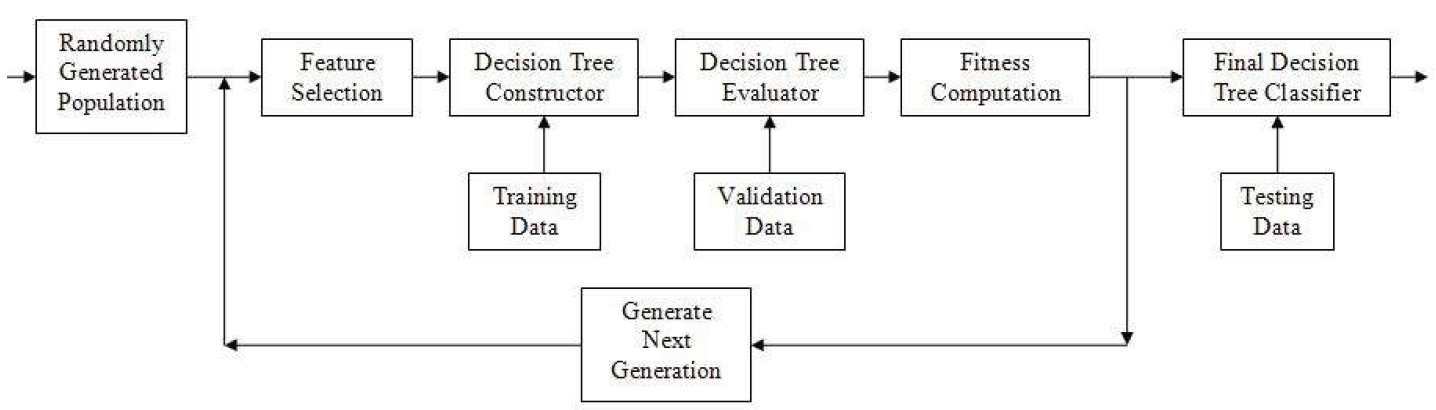
\includegraphics[scale=0.25]{dfd.png}
\caption{The data flow in DT/GA Hybrid Classifier.}
\end{figure}

In this algorithm, the search component is a GA and the
evaluation component is a decision tree. A detailed description of
this algorithm is shown in Figure 1. The basic idea of our hybrid system is to use GAs to
efficiently explore the space of all possible subsets of a given
feature set in order to find feature subsets which are of low
order and high discriminatory power. In order to achieve this
goal, fitness evaluation has to involve direct
measures of size and classification performance, rather than
measures such as the ranking methods such as information gain, etc.


The initial population is
randomly generated. Every individual of the population has N
genes, each of which represents a feature of the input data and
can be assigned to 1 or 0. 1 means the represented feature is used
during constructing decision trees; 0 means it is not used. As a
result, each individual in the population represents a choice of
available features. For each individual in the current population, a
decision tree is built using the ID3 algorithm. This resulting
decision tree is then tested over validation data sets, which
generate classification error rates. The fitness of this
individual is the weighted average of these classification error rates.
The lower the classification error rate, the better the fitness of the
individual.
Once the fitness values of all individuals of the current population
have been computed, the GA begins to generate next generation
as follows:
\begin{enumerate}
\item{}Choose individuals according to Roulette Selection method.
\item{}Use two point crossover to exchange genes between parents to
create offspring.
\item{}Perform a bit level mutation to each offspring.
\item{}Keep two elite parents and replace all other individuals of
current population with offspring.
\end{enumerate}
The procedure above is iteratively executed until the maximum
number of generations is reached or a Fitness value threshold, defined by the user, is crossed \textit{(in case the user doesn't want to wait for the algorithm to converge precisely)}. Finally, the best
individual of the last generation is chosen to build the final
decision tree classifier, which is tested on the test data set, and this is the tree that is returned.

\section{Object-Oriented Design and Results}
The decision tree based classifier was implemented in Java. The implementation is generic so that it can be applied to any supervised classification problem.


Object-oriented programming (OOP) is a programming paradigm that represents concepts as "objects" that have data fields \textit{(attributes that describe the object)} and associated procedures known as methods. Objects, which are instances of classes, are used to interact with one another to design applications and computer programs.
\\Had it not been for the presence of the OOP paradigm, our efforts in this project would have gone in vain, and we do not use that term lightly. Code management was a whole lot easier when compared to our past experience with procedural programming. In this section, we describe the different packages that were created by us to efficiently manage our code.\\
Know first that our application consists of four diverse packages. We describe each package in detail, in the following sections. We follow a bottom-up methodology for explaining the layout of the classes.

\begin{enumerate}
\item{\textbf{org.ck.sample}} - 
This package allows us to efficiently manage and encapsulate the details of the data samples, provided by users, which are required for analysis. It is this class that allows our application to accept generic data sets. It consists of five classes:

\begin{enumerate}
\item{\textbf{DataHolder}} - This class keeps track of names of files that contain training and testing samples; lists of features; their corresponding classification values; and Probability values. It provides this information, when required, to the front-end or back-end of our application. To make a long story short, this class acts like a middleman between the back-end and front-end of our application.
\item{\textbf{Feature}} - This class stores a mapping between a feature name and a feature value.

\item{\textbf{Sample}} - This class stores all the features and the corresponding classification value for one training/test sample only.  

\item{\textbf{SampleCollection}} - A SampleCollection, as the name suggests, is a collection of samples. In essence, this class reads the sample data from a file (using information provided by a DataHolder object) and initializes all the necessary data structures to store the data values for Classification analysis.

\item{\textbf{SampleSplitter}} - This class contains methods that operate on a given SampleCollection, in order to split it into two new SampleCollections, based on a given Feature. It also calculates the information gain of the given split operation.


\end{enumerate}




\item{\textbf{org.ck.dt}} - This package allows us to efficiently manage and encapsulate methods for all stages of Decision Tree Learning.

\begin{enumerate}

\item{\textbf{DecisionTreeNode}} - A DecisionTreeNode is a structure which may have either:

\begin{enumerate}
\item{a classification value, if it happens to be a leaf node}
\item{a list of one or more children DecisionTreeNodes, if it happens to be a decision node, i.e., an internal node.}
\end{enumerate}

Know that the types of these nodes is defined by the decision tree that is constructed, and a node has at most one parent.

\item{\textbf{DecisionTreeConstructor}} - This class takes a SampleCollection \textit{(containing training samples)} as input,  builds a decision tree and stores the root DecisionTreeNode of the decision tree. In essence, a DecisionTreeConstructor consists of a number of DecisionTreeNodes.

\item{\textbf{DecisionTreeClassifier}} - This class keeps track of the measurements of the DecisionTree constructed by a DecisionTreeConstructor object. It keeps track of the training as well as the test SampleCollection, and runs each sample through the Decision Tree that was constructed, to find out its classification accuracy, which it stores and retrieves, when required.


\item{\textbf{Discretizer}} - This class provides implementations of algorithms used for discretization. As mentioned earlier, decision trees work with discretized values, and if continuous-valued features are present, they have to be discretized. The Discretizer class contains two algorithms for discretization:
\begin{enumerate}
\item{A naive discretizer that discretizes data based on the median, with those values below the median being set to 0 and those values above the median being set to 1.}
\item{An Equal-Binning Discretizer that discretizes the values of certain feature of a collection of samples, by putting each value into particular bins. After discretization, the values can be any integer between 0 and binSize (inclusive).}
\end{enumerate}

\end{enumerate}



\item{\textbf{org.ck.ga}} - This package takes care of all operations of the Genetic algorithm that was mentioned earlier.

\begin{enumerate}
\item{\textbf{Genome}} - This class takes as input, a SampleCollection, and initializes a chromosome with random values for the presence/absence of features, as defined in Chapter 5. It keeps track of this chromosome, and provides methods to manipulate this chromosome; to calculate the fitness score of this chromosome; and to throw an exception when the fitness value threshold has been crossed or when the best solution has been discovered. It also provides facilities to switch between a chromosome and the corresponding optimal decision tree to which it is bound.


\item{\textbf{Population}} - As defined earlier, a population is a collection of genomes. And this is exactly what this class is. Initially, the Population class randomly initializes a large number of genomes, of which it keeps track. It provides methods such as roulette selection, reproduction, crossover, and mutation to operate on the population and discover the best genome, and hence, the best decision tree with the appropriate feature subset.

\item{\textbf{OptimalScoreException}} - This class is responsible for catching the best genome as soon as it is discovered, since the best genome should never be allowed to escape. It should be caught and nurtured for future use.

\end{enumerate}


\item{\textbf{org.ck.gui}} - As you've probably guessed by now, this package handles the Graphical User Interface of our application, with all its bells and whistles. We made use of the Standard Widget Toolkit for the GUI of our application. This package consists of the following classes:

\begin{enumerate}

\item{\textbf{WelcomeWindow}} - This class takes care of drawing the window that appears when our application is first switched on, and obviously, its name should be WelcomeWindow, nothing more, nothing less. It displays a list of clickable options, namely
\begin{enumerate}
\item{Train Decision Tree}
\item{Classify Data Sets}
\item{View on Github}
\item{Exit Application}
\end{enumerate}

We have organized the code in this package in such a way that all the options \textit{(except for the last one - "Exit Application")}, correspond to a different class which handles the creation of the corresponding window.

\item{\textbf{MainWindow}} - This class manages the window that is opened when a user clicks the \textit{Train Decision Tree} option in the Welcome Window. In this window, the user can select the appropriate options required to construct a decision tree using our Hybrid DT/GA Classifier. By the way, did we mention that a constructed decision tree can be saved for later usage?

\item{\textbf{ClassifyWindow}} - This class manages the window that is opened when a user clicks the \textit{Classify Data Sets} option in the Welcome Window. A user is provided with an interface to select a saved decision tree, and classify new samples based on it. It really saves a lot of time in this fast-paced world of ours.


\item{\textbf{BrowserWindow}} - This class manages the window that is opened when a user clicks the \textit{View on Github} option in the Welcome Window. In order to see and verify whether our code is original or not, users can see the online repository of our code (including its version history) on Github, in this window. Verification couldn't have been more easier. 

\item{\textbf{Constants}} - This interface (mark my words, this is not a class) contains a list of constants used by all the classes in all the packages. This interface really makes updating our software and meddling with various values much easier, like never before.



\item{\textbf{MainClass}} - Before our application had a GUI, this class was used to test out the code in the other packages using the console. The SampleCaller2 method is still being used by the MainWindow class. We didn't have the heart to delete this class, which has been with us for so very long. We kept it for old times' sake.



\end{enumerate}




\end{enumerate}







The DT/GA hybrid classifiers were tested with three classification problems, namely:
\begin{itemize}
\item{Classifying Horse blood samples}
\item{Determining the potability of water}
\item{Determining the quality of the wine}
\end{itemize}

The results of the GA-based optimization scheme is shown in the Figure 2.
\begin{figure}[h!]
  
  \centering
    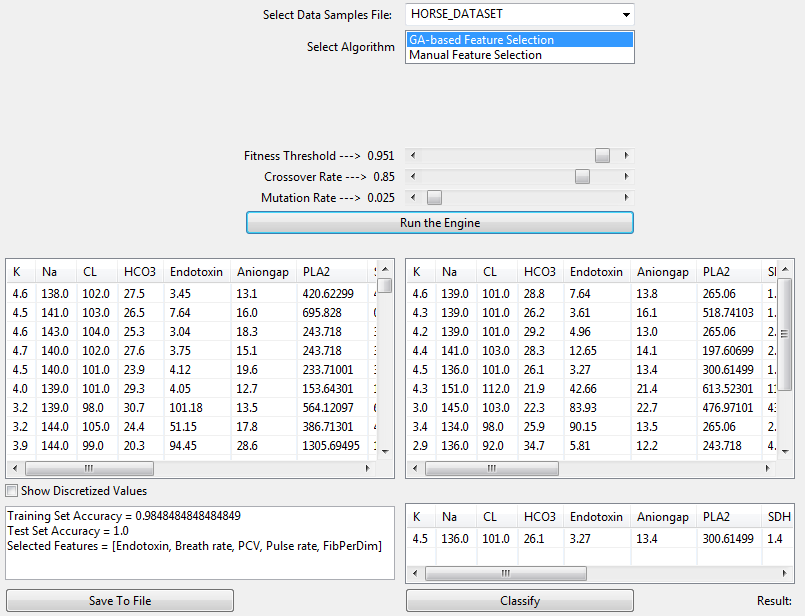
\includegraphics[scale=0.4]{ga_algo_stats.png}
\caption{DT built with GA based feature selection.}
\end{figure}

The results obtained with manual feature selection is shown in Figure 3.
\begin{figure}[h!]
  
  \centering
    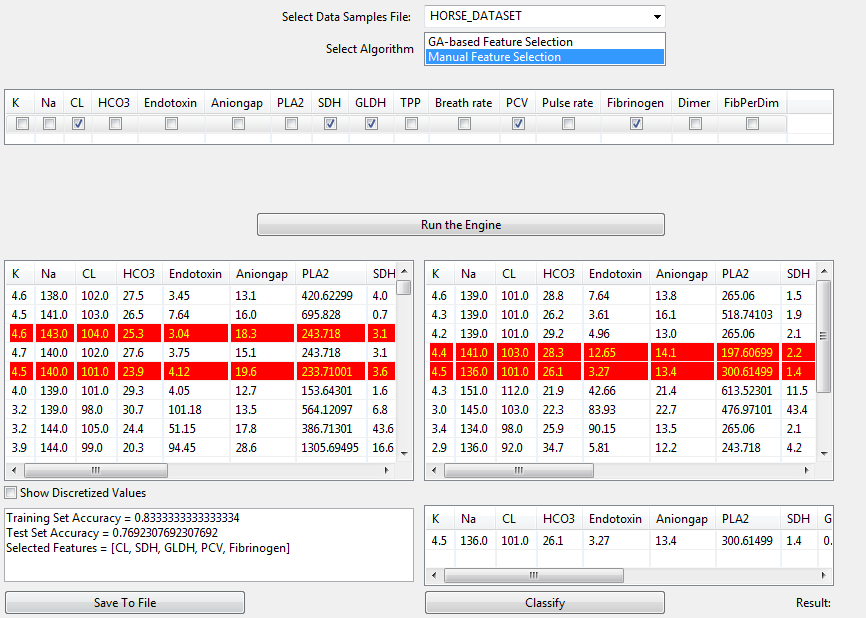
\includegraphics[scale=0.3]{manual_sel_stats.png}
\caption{DT built with manual feature selection.}
\end{figure}
\section{Conclusion}
The genetic algorithm and decision tree hybrid was able to
outperform the decision tree algorithm which was based on manual feature selection.
We believe that this improvement is due to the fact that the
hybrid approach is able to focus on relevant features and
eliminate unnecessary or distracting features. This initial filtering
is able to improve the classification abilities of the decision tree.
The algorithm does take longer to execute than the standard
decision tree; however, its non-deterministic process is able to
make better decision trees. The training process needs only to be
done once. The classification process takes the same amount of
time for the hybrid and non-hybrid systems.

\section{Future Work}
The hybrid GA /decision tree algorithm needs to be tested
further to realize its true potential. Clearly more work needs to be done. 
The test results show that the Decision Trees constructed using the Genetic algorithm-based feature selector, were more efficient and accurate in classifying the data than the Decision Trees constructed by selecting features manually. A forest of decision trees will be
constructed from the combination of four final decision trees,
each for one major attack category. The final decision will be
made through a voting algorithm. We will then compare the
overall classification ability of the hybrid algorithm with other
machine learning algorithms in the literature.

Some other future enhancements could include one of the following:
\begin{enumerate}
\item{The application could be made more responsive by using Threads and Parallel/Cloud Computing}
\item{The Decision Tree Classifier of this application could be optimized using Neural Networks which are more efficient than Decision Trees.}
\item{An interesting extension to be explored is the possibility of
additional feedback from ID3 concerning the evaluation of a
feature set. Currently only classification accuracy is returned.
However, there is potentially exploitable information with
respect to which features were actually used to build the
decision tree and their relative positions in the tree.}

\end{enumerate}


\begin{thebibliography}{1}

\bibitem{textbook}
Hua;Kien A., Wu;Annie S.; Chen;Bing, Stein;Gary
\emph{Decision Tree Classifier For Network Intrusion Detection
With GA-based Feature Selection}

\bibitem{paper}
Jing Xu, Ming Zhao,José Fortes, Robert Carpenter,
Mazin Yousif. \emph{Autonomic resource management in virtualized data centers using
fuzzy logic-based approaches} Cluster Comput (2008) 11: 213–227
DOI 10.1007/s10586-008-0060-0
\bibitem{paper}
T. Wood et al., \emph{Sandpiper.Black-box and gray-box resource management for virtual machines}, Computer Network (2009), doi:10.1016/j.comnet.2009.04.014
\end{thebibliography}

\end{document}


